\section{9/17/2019: Finite-Sample Concentration via Expanding the Set}

\subsection{Logistics}

\begin{itemize}
  \item HW1 due, separate document for challenge problem
  \item Can we help prof preserve references but split notes?
\end{itemize}

\subsection{Outline}

Previously, MDF
\begin{align}
  \hat\theta(\tilde{p}) &= \theta^*(q) = \min_\theta L(q,\theta) \\
  q &= \argmin_{q \in \cG} D(\tilde{p}, q)
\end{align}

Issue: if $\tilde{p} = \tilde{p}_n$ discrete, can fail.

Solution: Replace $D$ with $\tilde{D}$, or expand $\cG$ to $\cM$.
We saw $D = \TV$ and $\tilde{D} = \tilde{TV}_\cH$ the generalized KS distance
from last time
\begin{align}
  \tilde{\TV}_\cH = \left(\eps + \sqrt{\frac{d}{n}})\right)^{1 - 1/k}
\end{align}
for bounded $k$th moments.

WANT: $\eps^{1 - 1/k} + \sqrt{d/n}$.

By expanding to $\cM$, we mean
\begin{align}
  q = \argmin_{q \in \cM} \tilde{D}(\tilde{p}, q)
\end{align}

Outline for today:
\begin{itemize}
  \item True ``empirical distribution''
  \item Expand the set idea
  \item Analyze concentration for bounded $k$th moments
    \begin{itemize}
      \item symmetrization
      \item truncated moments
      \item ledoux-talagrand
    \end{itemize}
\end{itemize}

\subsection{True Empirical Distribution}

Let $p_n^*$ define an empirical distribution drawn from $p^*$.

\begin{figure}[H]
\begin{center}
  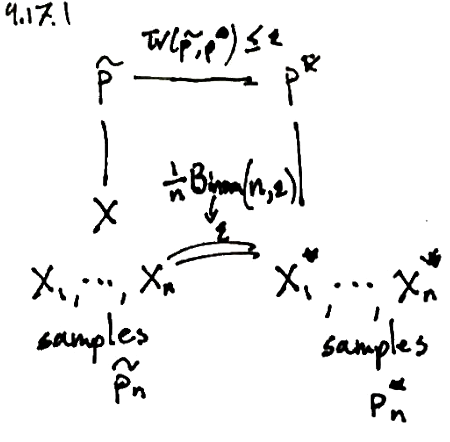
\includegraphics[width=0.3\textwidth]{figures/9-17-1.png}
\end{center}
\end{figure}


\textbf{Issue}: No overlap between $\tilde{p}_n$, $p_n^*$

\textbf{Solution}: Define \emph{coupling} between $p_n^*$ and $\tilde{p}_n$.

\begin{figure}[H]
\begin{center}
  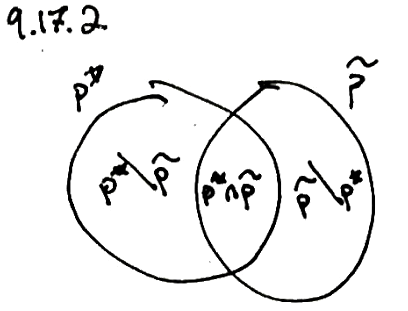
\includegraphics[width=0.3\textwidth]{figures/9-17-2.png}
\end{center}
\end{figure}

with probability $1 - \eps$
\begin{itemize}
  \item Sample from $p^* \cap \tilde{p}$, $X_i = \tilde{X_i} =$ sample
\end{itemize}
and with probability $eps$
\begin{itemize}
  \item Sample $X_i^*$ from $p^* \setminus \tilde{p}$
  \item Sample $X_i$ from $\tilde{p} \setminus p^*$
\end{itemize}

\textbf{Takeaway}:
$\underbrace{\TV(\tilde{p}_n, p_n^*)}_{\tilde{\eps}} \sim \frac{1}{n}\text{Binom}(n, \eps)$

\begin{lemma}[Tail bound for binomials]
  With probability $\geq 1 - \delta$
  \begin{align}
    \frac{1}{n} \text{Binom}(n, \eps)
    \leq O\left(\sqrt{\eps} + \sqrt{\frac{\log \frac{1}{\delta}}{2 n}}\right)^2
    = O\left(\eps + \frac{\log \frac{1}{\delta}}{2 n}\right)
  \end{align}
\end{lemma}

\begin{remark}
  This is tighter than Hoeffding, which would have given $\exp(-\eps^2 n / 3)$.
  Need Bernstein's inequality and Chernoff bound for binomial random variables
  to prove this.
\end{remark}

\subsection{Expanding the set idea}%

Fig 9.17.3:

Need three properties for $\cM$
\begin{itemize}
  \item $\cM$ large: $p_n^* \in \cM$ whp
  \item $\cM$ small: modulus $\fm(\cM_{\eps})$ small
  \item $p_n^*$ good approx to $p^*$: $\|\mu(p^*) - \mu(p_n^*)\|_2$ bounded
\end{itemize}

\begin{proposition}\label{prop:projection-bound-expand-G-to-M}
  Suppose
  \begin{itemize}
    \item $p^*_n \in \cM$ wp $1 - \delta$
    \item $\TV(p_n^*, \tilde{p}_n) \leq \tilde{\eps}$ wp $1 - \delta$
  \end{itemize}
  Then projecting onto $\cM$ yields $q$ where
  \begin{align}
    \|\mu(q) - \mu(p^*)\|_2 \leq \fm(\cM, 2 \tilde{\eps}) + \|\mu(p^*) - \mu(p_n^*)\|_2
  \end{align}
  wp $1 - 2 \delta$.
\end{proposition}

\begin{proof}
  Since $p_n^* \in \cM$, we have
  \begin{align}
    \TV(\tilde{p}_n, q) &= \min_{q \in \cM} \TV(\tilde{p}_n, q) \leq \tilde{\eps}
  \end{align}
  Also by hypothesis $\TV(\tilde{p}_n, p_n^*) \leq \tilde{\eps}$, so
  by triangle inequality
  \begin{align}
    \TV(p_n^*, q) \leq 2 \tilde{\eps}
  \end{align}
  Since $\|\mu(p_n^*) - \mu(q)\|_2 \leq \fm(\cM, 2\tilde{\eps})$ by definition
  (\cref{prop:mdf-modulus-error-bound}), we have
  by triangle inequality
  \begin{align}
    \|\mu(p^*) - \mu(q)\|_2 \leq \fm(\cM, 2 \tilde{\eps}) + \|\mu(p^*) - \mu(p_n^*)\|_2
  \end{align}
\end{proof}

\begin{example}[Bounded $k$th moments]
  Let
  \begin{align}
    \cG = \cG_k(sigma)
    &= \{ p : \lvert \ex X \rvert_{\psi_k} \leq \sigma \} \\
    &= \{ p : \ex_p[ \lvert \braket{X - \mu, v} \rvert^k] \leq \sigma^k~\forall \|v\|_2 \leq 1\}
  \end{align}
  where $\psi_k(x) = x^k$. Note $\cG_2(\sigma)$ are the distributions with
  bounded covariance \cref{corr:mod-cont-cov}.

  \textbf{Isuse}: $p_n^* \not\in \cG$ until $n \gg d^{k/2}$. For example,
  $p^* = \cN(\mu, I)$ has
  \begin{align}
    \ex_{p_n^*}[\lvert \braket{X - \mu, v}\rvert^k]
    \geq \frac{1}{n} \lvert \braket{x_1 - \mu, v}\rvert^k
  \end{align}


  \begin{figure}[H]
    \begin{center}
      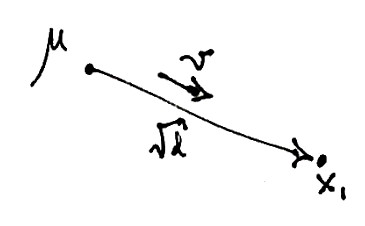
\includegraphics[width=0.3\textwidth]{figures/9-17-4.png}
    \end{center}
  \end{figure}
  Figure 9.17.4: $\frac{1}{n} \lvert \braket{X_1 - \mu, v}\rvert^k = \frac{1}{n} \underbrace{\|X_1 - \mu\|_2^k}_{\sqrt{d}} = \left( \frac{1}{n} d^{k/2} \right)^{1/k} = \frac{\sqrt{d}}{n^{1/k}}$.

  ``Moment along a single direction of a sample is large, need to average over
  many before it washes out''
\end{example}

Consider expanding bounded $k$th moments $\cG = \cG_k(\sigma)$ to the larger
set of resilient distributions $\cM = \cG_{\TV}(\rho, \eps)$ with $\rho = O(\eps^{1 - 1/k})$.

To use \cref{prop:projection-bound-expand-G-to-M}, we need to show two easy
things:
\begin{itemize}
  \item Bound modulus $\fm(\cM, \eps) \leq 2 \rho = O(\eps^{1 - 1/k})$
  \item Bound $\|\mu(p^*) - \mu(p_n^*)\|_2 = O\left(\sigma \sqrt{\frac{d}{n} \delta^{-1/k}}\right)$
\end{itemize}
and one hard thing
\begin{itemize}
  \item Show $p^*_n \in \cM$.
\end{itemize}

\begin{lemma}
  \begin{align}
    \|X\|_2 &= \ex_{v \sim \cN(0,I)}[\lvert\braket{x,v}\rvert] \sqrt{\frac{\pi}{2}}
  \end{align}
\end{lemma}
\begin{proof}
  \begin{align}
    \ex[\lvert
    \braket{
      (\|x\|_2, 0, \ldots, 0),
      (v_1,\ldots, v_d)
    } \rvert]
    = \ex[\lvert v_1 \rvert \cdot \|x\|_2] \\
    \ex[\lvert v_1\rvert] = \sqrt{2/\pi}
  \end{align}
\end{proof}

\begin{remark}
  There's a better version of the above called \emph{Khintchine's inequality}:
  \begin{align}
    \|X\|_2 \leq \sqrt{2} \ex[\lvert \braket{X, \eps} \rvert]
  \end{align}
  with $\eps \sim \text{Rad}$. So we can just test using Rademachers rather
  than Gaussian process.
\end{remark}

\todo{We failed to prove the second easy thing in class using above, see notes
for update}

Now we show $p_n^* \in \cM$, introducing some new ideas along the way.

\subsubsection{Truncated moments}

\textbf{Problem}: $\| \cdot \|_{\psi_k}$ is not small.

\textbf{Solution}: Truncate moments, replace $\psi_k(x) = x^k$ with
\begin{align}
  \tilde{\psi}_k(x) = \begin{cases}
    x^k & x \leq x_0 \\
    k x_0^{k-1} (x - x_0) + x_0^k : x > x_0
  \end{cases}
\end{align}


\begin{figure}[H]
\begin{center}
  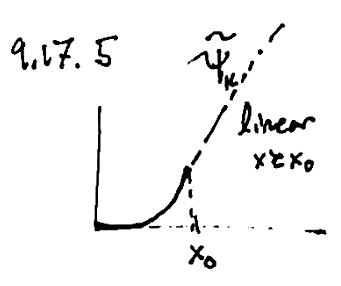
\includegraphics[width=0.3\textwidth]{figures/9-17-5.png}
\end{center}
\end{figure}

$\tilde{\psi}_k$ is $L$-Lipschitz, for $L = k x_0^{k-1}$.
$x_0 = \left(\frac{1}{\eps}\right)^{1/k}$, $L = k / \eps^{1 - 1/k}$.

\begin{proposition}\label{prop:truncated-moments-bound}
  Let $X_1, \ldots, X_n \sim p^*$, where $p^* \in \cG_k(\sigma)$. Then
  \begin{align}
    \ex_{X_i \sim p^*}\left[
      \sup_{\|u\|_2 = 1} \frac{1}{n} \sum_{i=1}^n \tilde{\psi}_k\left(
        \left\lvert \frac{\braket{X_i - \mu, v}}{\sigma}\right\rvert
      \right)
    \right]
    &\leq 1 + 2 L \sqrt{\frac{d}{n}}
  \end{align}
  where $L = k x_0^{k-1}$.
\end{proposition}

\begin{remark}
  When  $n \geq 4 L^2 d = 4 k^2 d / \eps^{2 - 2/k}$, we have
  \begin{align}
    \sup_{\|u\|_2 = 1} \frac{1}{n} \sum_{i=1}^n \tilde{\psi}_k\left(
      \left\lvert \frac{\braket{X_i - \mu, v}}{\sigma}\right\rvert
    \right)
    \leq 2
  \end{align}

  This implies that $p_n^*$ has bounded Orlicz norm
  $\|p_n^*\|_{\tilde{\psi}_k}$, so by \cref{lem:orlicz-norm-resilient}
  $p_n^*$ is resilient with parameter $\sigma \eps \tilde{\psi}^{-1}(2/\eps)$.

  So we really need to control how fast $\sigma \eps \tilde{\psi}^{-1}(2/\eps)$
  grows.


\begin{figure}[H]
\begin{center}
  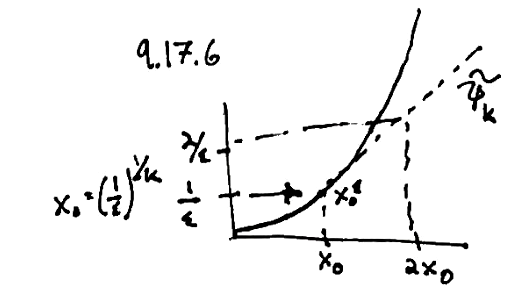
\includegraphics[width=0.3\textwidth]{figures/9-17-6.png}
\end{center}
\end{figure}
$\sigma \eps \tilde{\psi}^{-1}(2/\eps) \leq 2 \sigma
  \eps \underbrace{\left(\frac{1}{\eps}\right)^{1/k}}_{> 0}
  = 2 \sigma \eps^{1 - 1/k}$
\end{remark}

\subsubsection{Ledoux-Talagrand contraction}%

This result is used as part of symmetrization arguments. If I have already symmetrized and I have
a Lipschitz function, than I can always repalce the function with just its
arguments and make things bigger.

\begin{theorem}[Ledoux-Talagrand]
  \begin{align}
    \ex_{\eps}\left[
      \sup_{v \in V} \frac{1}{n} \sum^{n}_{i=1} \eps_i \phi(\braket{x_i, v})
    \right]
    \leq \ex_\eps\left[
      \sup_{v \in V} \frac{1}{n} \sum_{i=1}^n \eps_i \braket{x_i, v}
    \right]
  \end{align}
  for $\phi$ $1$-Lipschitz, i.e. $\vert \phi(x) - \phi(y) \rvert \leq \lvert x - y \rvert$,
  $V$ a symmetric set, and $\eps \sim \text{Rad}$.
\end{theorem}

\begin{proof}[Proof of \cref{prop:truncated-moments-bound}]
  \begin{align}
    &\ex_{X_i \sim p^*}\left[
      \sup_{\|u\|_2 = 1} \frac{1}{n} \sum_{i=1}^n \tilde{\psi}_k\left(
        \left\lvert \frac{\braket{X_i - \mu, v}}{\sigma}\right\rvert
      \right)
    \right] \\
    &= \underbrace{\ex[\tilde{\psi}]}_{\leq \ex\psi \leq 1} + \sup_{\|v\|_2 \leq 1} \frac{1}{n} \sum^{n}_{i=1} \left(
      \tilde{\psi}_k(\lvert \braket{x_i - \mu, v} / \sigma \rvert) - \ex[\tilde\psi]
    \right)
  \end{align}

  \begin{align}
    \ex_{X_i, X_i' \sim p^*, \eps \sim \text{Rad}}\left[
      \sup_{\|v\|_2 \leq 1} \frac{1}{n} \sum^{n}_{i=1}
      \eps_i \left(
        \tilde{\psi}_k\left(\frac{\lvert \braket{X_i - \mu, v}\rvert}{\sigma}\right)
        -  \tilde{\psi}_k\left(\frac{\lvert \braket{X_i' - \mu, v}\rvert}{\sigma}\right)
      \right)
    \right]
  \end{align}
\end{proof}
